\part{Administración de entrada/salida}

\section{Subsistema de I/O}
Los elementos básicos de hardware, como puertos, buses y controladores se conectan una gran variedad de disposivitos de entrada/salida que varian en sus funciones y velocidades por lo que se necesitan varios métodos para controlarlos. Éstos forman parte del \textbf{subsistema de I/O} y son encapsulados en módulos llamados \textbf{drivers}. 

Los drivers presentan una interfaz de acceso uniforme a los subsitemas de entrada/salida, eliminando la necesidad de que el sistema operativo sepa como manejar las particularidades de cada dispositivo. Los mismos corren con máximo privilegio y de ellos depende el rendimiento de todo el subsistema de entrada/salida

La mayoría de los dispositivos que se usan en una computadora pueden ser clasificado como de almacenamiento (discos, memorias flash), de transmissión (conexiones al internet, bluetooth) e interface de usuarios (pantallas, teclados, mouse).

\paragraph{Puerto (Port):} Es un cable mediante el cual se comunican los dispositivos de entrada/salida con el sistema

\paragraph{Bus:} Es un conjunto de cables compartidos por varios dispositivos junto con un protocolo específico que define un conjunto de mensajes que pueden ser enviados a los mismos.

\paragraph{Controlador:} Es un dispositivo que puede operar un puerto, un bus u otros dispositivos. Algunos controladores pueden llegar a tener un pequeño procesador, microcodigo y memoria privada integradas para implementar protocolos complejos. Un ejemplo de esto son los controladores \textbf{Small Computer System Interface (SCSI)} que se encargan de comunicar los discos con el sistema

\begin{figure}[h]
	\centering
	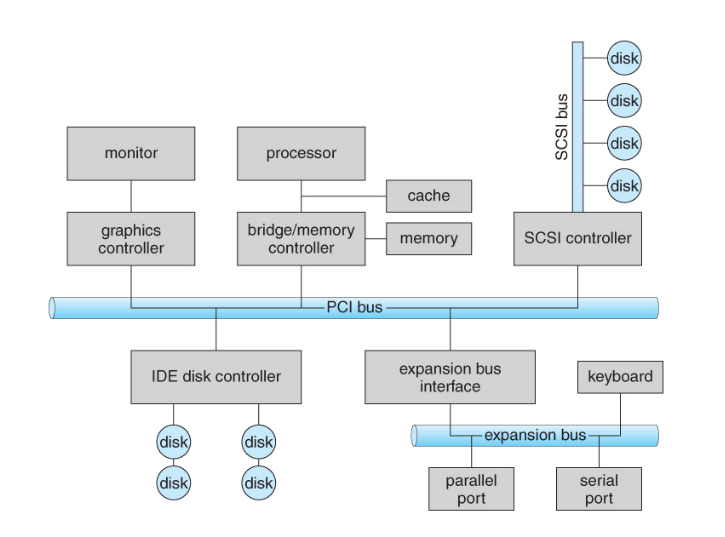
\includegraphics[width=0.5\textwidth]{imagenes/estructura-basica-bus}
	\caption{Estructura típica de un Bus}
	\label{fig:estructura-basica-bus}
\end{figure}

\subsection{Interacción con los dispositivos}
La interacción entre el sistema y un controlador puede tomar varias formas. La más simple es conocida como \textbf{polling} o \textbf{busy-waiting}. Con este método, el sistema está constantemente verificando el estado de un dispositivo hasta que está listo para ser usado. Una vez que el dispositivo está listo, le manda un pedido y vuelve al ciclo de verificación hasta que el dispositivo marca que el pedido fue atendido.

Esté método tiene sentido en dispositivos que deben ser atendidos rápidamente. Por ejemplo,el buffer de los controladores de teclados es muy pequeño y podríamos perder información si el sistema tarda demasiado en leer los bytes del mismo.

Sin embargo es ineficiente cuando el dispositivo se usa poco y hay otros procesos que deben terminarse. En estos casos es más eficiente configurar los controladores para que notifiquen al CPU cuando el dispositivo está listo para atender un pedido. El mecanismo que permite implementar esto es llamado \textbf{interrupciones}.

\subsubsection{Interrupciones}
El CPU tiene un cable llamado linea de pedido de interrupciones (\textbf{interrupt-request line}) que se chequea cada vez que se termina de procesar una instrucción. Cuando se detecta una interrupción en este cable, el sistema determina cuál fue la causa, realiza el procesamiento necesario para atenderla y luego sigue ejecutando los procesos del usuario.

\subsubsection{Direct Memory Access}
Para dispositivos que realizan transferencias de grandes cantidades de datos, como discos rígidos, se usa un procesador especial llamado controlador de acceso directo a memoria (\textbf{Direct Memory Access Controller}).

El sistem debe avisarle al controlador DMA que desea realizar una transferencia y le pasa un puntero a la data que quiere transferir, un puntero a donde quiere hacerlo y la cantidad de bytes que deben ser transferidos. El controlador procede a realizar la transferencia mientras el CPU pasa a otra tareas por lo que no es necesario esperar a que termine la transferencia para seguir trabajando.

\subsection{Drivers}
Podemos abstraer las diferencias especificas entre los dispositivos de entrada/salida clasificandolos de una manera más generalizada. Cada clase es accedida a través de una conjunto estandarizado de funciones (una \textbf{interfaz}) que debe ser implementada por los drivers de cada dispositivo.

Las interfaces presentadas por el sistema deben en tener en cuenta las siguientes características de los dispositivos:

\begin{itemize}
	\item \textbf{Tamaño de transferencia } (character-stream or block-steram): Los dispositivos \textbf{character-stream} transfieren byte a byte, mientras que los dispositivos de transferencia bloques transmiten una unidad de información compuesta de varios bytes.
	\item \textbf{Acceso secuencial o aleatorio}: Un dispositivo secuencial transfiere información en un orden determinado por el dispositivo, mientras que los usuarios de un dispositivo de acceso aleatorio pueden pedir que se busque cualquier porción de la memoria disponible.
	\item \textbf{Sincróno o asincróno:} Un dispositivo síncrono realiza las transferencia con un tiempo de respuesta predecible y coordina con otros aspectos del sistema. Un dispositivo asíncrono exhibe tiempos de respuesta irregulares que no se pueden coordinar con otros eventos del sistema.
	\item \textbf{Compartido o dedicado:} Un dispositivo compartido puede ser usado por varios procesos o thread de manera concurrente, mientras que uno dedicado no. 
	\textbf{Velocidad de operación:} Puede variar de uno pocos bytes por segundo a varios gigabytes por segundo, dependiendo el dispositivo.
	\textbf{Tipo de comunicación:} Puede ser dispositivos de solo escritura, de solo lectura o de escritura/lectura.
\end{itemize}

\subsubsection{Block devices}
La interfaz de los dispositivos de bloque capturan todos los aspectos necesarios para acceder a dispositivos de almacenamiento. Los comandos básicos que se espera que respondan son: \texttt{read()} y \texttt{write()}. Además de la operación \texttt{seek()}si el dispositivo permite acceso aleatorio.

Sin embargo, hay aplicaciones especiales (como los motores de bases datos) que pueden preferir acceder a los dispositivos como si fuesen un arreglo lineal de bloques (\textbf{raw I/O}) debido a que implementan sus propios buffers o técnicas de escrituras. Por estar razón, se permite a esos programas realizar los accesos directos y evitar el comportamiento default del sistema operativo.

\subsection{Spooling}
Su nombre proviene de \textbf{Simultaneous Peripheral Operation On-Line} y consiste en un buffer que almacena información que se debe enviar a un dispositivo, como una impresora, que no puede aceptar información de manera intercalada. Aunque una impresora puede ejecutar un solo trabajo por vez, varias aplicaciones pueden requerir su uso de manera concurrente y es necesario que sus salidas no se mezclen. El sistema operativo resuelve este problema interceptando todos los pedidos y enconlandolos en este buffer. Cuando la impresora está lista para responder un nuevo pedido, el sistema copia el siguiente archivo de la cola.

Hay que tener en cuenta que este proceso es visible a nivel usuario y es manejado por el sistema operativo. El kernel y los controladores actuan de manera normal.
 
\printbibliography[keyword=drivers, title=Bibliografía]

\newpage
\section{Almacenamiento Secundario}
\subsection{Tipos de discos}
\subsubsection{Discos Magnéticos}\label{discosMagneticos}
Son la mayor parte del sistema de memoria secundario en las computadoras modernas. Un disco rígido, consiste en un conjunto de platos (\textbf{platters}) con una forma circular y varios cabezales de lectura-escritura (\textbf{read-write head}) que ``vuelan" sobre su superficie:

\begin{figure}[h]
	\centering
	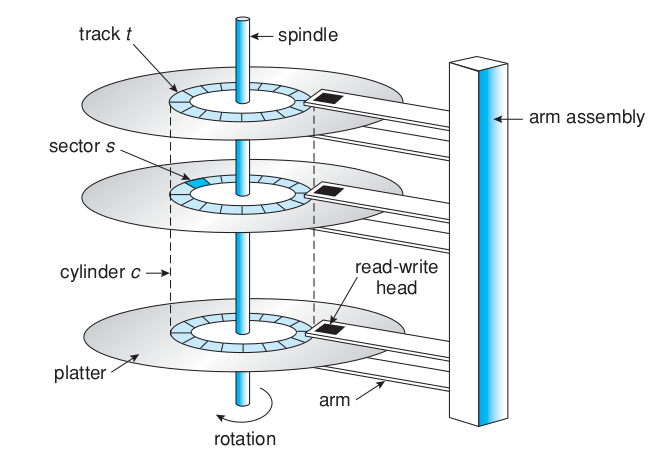
\includegraphics[width=0.7\textwidth]{imagenes/mecanismo-lectura-disco}
	\caption{Mecanismo de lectura/escritura de un disco}
	\label{fig:mecanismo-lectura-disco}
\end{figure}

Todos los cabezales están unidos a un brazo que los mueve de manera unísona. Cuando un disco está en uso, un motor gira sus platos a alta velocidad y el brazo mueve los cabezales de manera radial (desde el centro del plato hasta el perímetro del mismo y viceversa).

La superficie de cada plato está divida en sectores lógicos llamados \textbf{tracks} que están subdivido en \textbf{sectores}. El conjunto de \textbf{tracks} que estan a la misma distancia del brazo se llama \textbf{cilindro}. Cada disco puede tener miles de cilindros y cada track cientos de sectores por lo que en general la capacidad de estos dispositivos se mide en gigabytes.

La velocidad de un disco se divide en dos partes:
\begin{itemize}
	\item \textbf{Velocidad de transferencia (Transference Rate):} La velocidad a la que la infromación viaja entre el disco y la computadora.
	\item \textbf{Tiempo de posicionamiento (random-acces time):} Que es el tiempo que tarda el disco en encontrar un sector determinado. Este tiempo se puede dividir en dos partes:
	\begin{itemize}
		\item \textbf{Tiempo de búsqueda (seek time):} El tiempo necesario para mover el cabezal al cilindro adecuado.
		\item \textbf{Latencia rotacional (Rotational Latency):} El tiempo necesario para que el sector llegue al cabezal ya posicionado
	\end{itemize}
\end{itemize}
Generalmente, los discos pueden transferir varios megabytes de datos por segundo y los tiempos de búsqueda y de giro toman varios milisegundos.

Un disco puede ser removible permitiendo que varios discos se vayan montando y desmontando a medida que sea necesario. Algunas formas de discos removibles incluyen: CDs, DVDs y Blu Rays y memorias \textbf{flash}.

\subsubsection{Discos de estado solido (SSD)}
Un disco de estado sólido es una memoria no volátil que es usada como disco rígido. Tienen las mimas características que los discos clásicos pero son más seguros porque no tienen partes mobiles y son más rápidos por queno tienen latencia y ni tiempo de búsqueda. Además, consumen menos energía. Sin embargo, son más caros que los discos tradicionales, tienen menos capacidad y tiempos de vida más cortos.

Otro problema que tiene este tipo de discos es llamado \textbf{write amplification}, en el cual la cantidad de información escrita en el disco es un múltiplo de la cantidad lógica que se intentó escribir. En las memorias flash, es necesario borrar la memoria antes de poder escribirla pero las operaciones de borrado tienen una granularidad bastante mayor a la de escritura. Entonces, el proceso de escribir a memoria, muchas veces implica mover la sección usada de un bloque a alguna ubicación no usada del disco y luego borrar todo el bloque para luego poder escribir en la ubicación deseada.

Osea que una escritura puede requerir que se lea, actualize y reescriba alguna parte de la memoria ya utilizada en una nueva ubicación. Borrar la ubicación inicial y luego escribir los datos que se desean guardar. Este efecto multiplicador aumenta la cantidad de escrituras necesarias en el disco, lo que acorta el tiempo que puede funcionar de manera confiable.

\subsubsection{Cintas Magneticas}
Fueron de los primeros medios de almacenamiento utilizados. Aunque tienen una larga vida útil y tienen una gran capacidad de almacenamiento, sus tiempos de acceso son muchos mas lentos que la de los discos magnéticos.

\subsubsection{Almacenamiento virtual (Network-Attached Storage - NAS)}
Un dispositivo de almacenamiento virtual es sistema de almacenamiento que se accede remotamente desde una red de datos. Los dispositivos y sus usuarios están conectados a una red y se comunican mediantes paquetes TCP o UDP. Los clientes envian las las llamadas a los procedimientos que se deben realizar en algún dispositivo y luego los dispositivos le responden con la información pedida.

Este tipo de almacenamiento es una forma conveniente de compartir archivos y datos entre todas las computadoras de una red LAN. Sin embargo, tiende a ser menos eficiente que los dispositivos conectados fisicamente a cada computadora.
 
\subsubsection{Storage-Area Network (SAN)}
Son redes privadas que implementan protocolos específicos de almacenamiento y sirven para conectar servidores con unidades de almacenamiento. Estos protocolos, incluyen como repartir la memoria disponible entre multiples hosts y las políticas de uso de cada dispositivo de almacenamiento, etc.

\subsection{Politicas de Scheduling de E/S a disco}


Una de las respobilidades del sistema operativo es usar el hardware de manera eficiente. Para los discos magnéticos, esto es tener la responsabilidad de tener un tiempo de acceso rápido y conseguir un gran ancho de banda. 

\paragraph{Ancho de banda:} Es el número total de bytes transferidos divido el tiempo total transcurrido desde el primer pedido del servicio hasta que se termina de completar la transferencia.

\vspace*{5mm}
Cuando un proceso necesita realizar una operación de I/O en el disco, realiza una llamada al sistema operativo que especifica:
\begin{itemize}
	\item Si la operación es de entrada/salida.
	\item La dirección del disco desde con la que se debe realizar la transferencia
	\item La dirección de memoria principal a usar para la transferencia
	\item La cantidad de sectores que se deben transferir
\end{itemize}
Si el disco deseado y el controlador están disponibles, entonces el pedido se puede atender inmediatamente. Si alguno de los dos están ocupados, entonces se debe encolar en una cola de pedidos pendientes para ese disco. 

Una vez que el disco y el controlador están libres, el sistema operativo debe elegir cuál pedido atender:

\subsubsection{First-come, first-served (FCFS)}
El algoritmo más simple. Es intrisicamente justo pero no provee el servicio más rápido. Ya que dependiendo el orden en el que lleguen los pedidos puede ser que sea necesario mover el cabezal a través de todo el disco:

\begin{figure}[h]
	\centering
	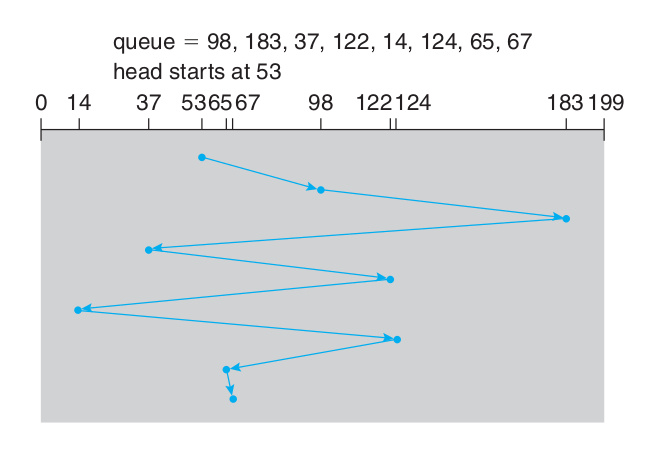
\includegraphics[width=0.7\textwidth]{imagenes/disco-fcfs}
	\caption{Recorrido del cabezal para algoritmo FCFS: El cabezal va desde el cilindro 53 hasta el 98, luego al 183, 37, 122, en orden hasta atender el último pedido en el cilindro 67. Se puede ver que si, en vez de haberlos hechos de esta manera, se hubiesen atendido primero el 37 y el 14 y después el 122 y el 124 también se hubiese reducido la distancia recorrida por el cabezal}
	\label{fig:disco-fcfs}
\end{figure}


\subsubsection{Shortest Seek Time First (SSTF)}
Se atienden primero los pedidos más cercanos al cabezal de escritura/lectura. 
Este algoritmo provee una sustancial mejora en el rendimiento del disco pero puede llegar a causar inanición de algunos pedidos, un escenario que se vuelve cada vez más probable a medida que la cola de espera crece.

\subsubsection{SCAN}
El brazo del disco comienza en un extremo del disco y se mueve hacia el final respondiendo pedidos a medida que va alcanzando cada cilindro. Una vez que termina de recorrer el disco, el brazo vuelve a repetir el proceso pero en la dirección inversa.

Si un pedido que esté justo enfrente del cabezal llega a la cola, entonces es resuelto inmediatamente. Si el cabezal ya pasó por ese sector, se deberá esperar a que el mismo llegue hasta el final del disco y vuelva hasta el sector correspondiente.

\subsection{Gestión del disco}
El sistema operativo también es responsable de manejar otros aspectos del disco:

\subsubsection{Formateo} 
Antes de porder guardar información en un disco, se lo debe dividir en sectores que el controlador del disco pueda leer y escribir. Este proceso es llamado \textbf{formateo de bajo nivel} o \textbf{formateo físico}. El formateo llena el disco con una estructura de datos especial para cada sector que consiste en un header, un área de datos y un \textit{posfijo}.

El header y el posfijo contienen información como el número del sectory codigo de corrección de errores. El controlador del disco actualiza esta información cada vez que realiza una escritura. Y la usa para comprobar que no haya fallas en ese sector cuando necesita leer del mismo. Si hay alguna falla, entonces puede usar el código de corrección de errores para recuperar la información corrupta. Sin embargo, esto solo es posible si solo fueron corrompidos uno pocos bits.

\subsubsection{Booteo} 
Cuando una computadora se enciende, necesita que se ejecute un programa llamado \textbf{bootstrap} que inicializa todos los aspectos del sistema (desde los registros de la CPU, los controladores de los dispositivos. el contenido de la memoria principal hasta el sistema operativo).

En la mayoria de las computadoras, se guarda un cargador de este programa (\textbf{bootsrap loader}) en una área de memoria de solo lectura (\textbf{read only memory - ROM}). El bootstrap loader se encarga de leer el programa de bootstrap desde disco. El mismo está ubicado en los bloques de inicialización (\textbf{boot blocks}) que están en una posición fija. 

\subsubsection{Bloques dañados}
Como los discos tienen partes movibles y tolerancias bajas, son propensos a fallas. En caso de que el fallo sea completo, el disco debe ser remplazado y no será posible recuperar su contenido a menos que se cuente con un disco de backup. 

En el caso de que solo haya sectores defectuosos, se pueden utilizar varias estrategias para manejarlos:
\begin{itemize}
	\item La más simple de todas, es escanear el disco para encontrar aquellos bloques defectuosos y marcarlos como inservibles para que el sistema operativo no los reserve.
	\item Otra técnica más sofisticada, es hacer que el controlador del disco mantenga una lista de los bloques defectuosos. Esta lista se inicializa durante el formateo de bajo nivel durante la fabriación y es actualizada constatemente durante la vida útil del disco.
	
	En este caso, el formateo genera sectores extra que no son visibles al sistema. De esta manera, cuando un bloque se daña, puede ser remplazado por uno de estos sectores sin mayores problemas.
\end{itemize}

\subsection{RAID}
Gracias a que los discos son cada vez mas baratos, es cada vez más factible tener varios discos en un sistema, lo que nos da la oportunidad de mejorar la velocidad de transferencia del sistema, y la seguridad de la información.

La solución para disminuir la probabilidad de perdida de datos, es agregar \textbf{redundancia}. Es decir, guardamos información que no es necesaria pero que puede usar en caso de que un disco falle para reconstruir la informción perdida.

La forma más simple (y más cara) de lograr esto es utilizar la técnica de \textbf{mirroring} que consiste en duplicar los datos de cada disco. En este caso, cada vez que se escribe algo a memoria, la operación se realiza en ambos discos por igual. Si algún disco falla, los datos pueden ser leídos del otro disco hasta que el disco dañado sea remplazado por uno nuevo.

Para mejorar la velocidad de transferencia se puede distribuir los bloques de un mismo archivo entre los discos. Está técnica es conocida como \textbf{\textit{data stripping}}. Cada disco participa en cada acceso a memoria 
lo que permite multiplicar la cantidad de información enviada por cada acceso de memoria.

Entonces \textbf{mirroring} provee alta seguridad de los datos pero es caro y \textbf{stripping} nos permite alcanzar altas velocidades de transferencia pero no mejora la seguridad. Por esta razón, se diseñaron varios esquemas que combinan estás dos técnicas de distintas maneras para lograr buenos trade-offs entre seguridad y ancho de banda.

Este conjunto de esquemas son conocidos como \textbf{Redundant Arrays of Independent Disks (RAID)} y están classificados en niveles:

\begin{itemize}
	\item \textbf{RAID 0 (Stripping):} Los bloques de un mismo archivo se distribuyen en dos (o más discos). No aporta ninguna redundancia, pero permite escrituras en paralelo lo que mejora el ancho de banda.
	\item \textbf{RAID 1 (Mirroring)}: Las escrituras se realizan en dos (o más) discos de manera simultanea. En el mejor de los casos tardan lo mismo que si tuviesemos un solo disco, en el peor tarda el doble. Mejora el rendimiento de las lecturas pero es demasiado caro de implementar.
	\item \textbf{RAID 2:} Tambien conocido como \textbf{memory-style error-correcting-code organizatio n(ECC)}. Se realiza un stripping a nivel bit de los datos que se guardan en discos distintos. Los códigos de corrección de error se guardan en discos aparte. Si un disco falla, entonces se puede usar el resto de los bits del archivo desde los otros discos y junto con su código de corrección correspondiente para recuperar la información perdida.
	\item \textbf{RAID 3:} Mejora el RAID 2 teniendo en cuenta que los controladores de disco pueden detectar si un sector fue leído correctamente por lo que un único bit de paridad puede ser usado tanto como para corregir como para detectar daños. Si uno de los sectores está dañado, sabemos que sector es y podemos calcular el valor del bit perdido a partir de la paridad de los sectores en los otros discos. Este tipo de RAID es igual de efectivo que el RAID 2 pero es más barato de implementar.
	
	Este nivel, es mejor que el nivel 1 porque se reduce la cantidad de discos necesarios para conseguir redundancia. Sin embargo, soporta menos operaciones de entrada/salida por segundo ya que todos los discos deben participar en cada transferencia. Además, puede llegar a ser muy caro computar la paridad de cada bloque.

	\item \textbf{RAID 4:} O \textbf{block-interleaved parity orgnaization} usa stripping a nivel de bloque, como raid 0, pero mantiene un disco a parte en el que se guarda bloques de paridad por cada bloque de los otros discos. Si un disco falla, se puede recuperar el bloque dañado usando los bloques del resto de los discos junto con el bloque de paridad.
	
	Un lectura accede solo un dico, por lo que es posible atender varios pedidos de manera simultanea por lo que el ancho de banda para lecturas es alto. Sin embargo, cuando se desean realizar escrituras de tamaños pequeños, es necesario cargar en memoria todo el bloque, modificarlo y luego volver a escribirlo en disco, además de actualizar el bloque de paridad. Esto puede alentizar el sistema.
	
	\item \textbf{RAID 5:} O \textbf{block-interleaved distributed parity} es el RAID 4 con la diferencia que los datos y los bloques de paridad se reparten entre todos los discos. Esto aligera la carga de los discos que hubiesen sido usados como discos de paridad, alargando su vida útil.
	
	\item \textbf{RAID 6:} Es como el RAID 5 pero almacena más información redudante para proteger de fallas de múltiples discos.
	
	\item \textbf{RAID 0 + 1:} Es una combinación de los RAID 0 y RAID 1. Se realiza un stripping de la data entre varios discos y luego se duplican esa escritura en otro conjunto de discos. Generalmente, tiene mejor performance que el RAID 5 pero duplica la cantidad de discos necesarios para implementarlo.
\end{itemize}

Por lo general, junto con estos esquemas se agrega un disco de respuesto que no es usado hasta que un disco falle completamente. Una vez que esto sucede, se reconstruye en el mismo la data perdida. Además RAID solo protege de errores físicos en los discos, no de errores  de otros hardware o software por lo que es necesario tener copias de seguridad y sistemas de archivos que brinden protección extra.

\printbibliography[keyword=discos, title=Bibliografía]

\newpage
\section{\red{Sistemas de archivos}}
\subsection{\red{Responsabilidades del FS}}
% TODO
\subsection{\red{Punto de montaje}}
% TODO
\subsection{\red{Representación de archivos}}
% TODO
\subsection{\red{Manejo del espacio libre}}
% TODO
\subsection{\red{FAT, inodos}}
% TODO
\subsection{\red{Atributos}}
% TODO
\subsection{\red{Directorios}}
% TODO
\subsection{\red{Caché}}
% TODO
\subsection{\red{Consistencia, journaling}}
% TODO
\subsection{\red{Características avanzadas}}
% TODO
\subsection{\red{NFS, VFS}}
% TODO
